\section{Simulation details}\label{app:simdetails}

This appendix documents the simulation study of \cref{sec:simulation}: the software and
the runs (\cref{app:sim-run}), the configurations (\cref{app:sim-config}), the estimator
settings (\cref{app:sim-est}), further results of E1, E4 and E5 (\cref{app:sim-e1e5}), the
Monte Carlo standard errors (\cref{app:sim-mcse}) and how to reproduce the results
(\cref{app:sim-repro}). All data are synthetic. Every configuration value below is stored
with the results in \texttt{results/sim\_results.json}, and the per-replicate values are in
\texttt{results/raw/E1.json}, \dots, \texttt{results/raw/E6.json}.

\subsection{Software, seeds and runs}\label{app:sim-run}

\paragraph{Software} The experiments are run by \texttt{code/run\_experiments.py}. It
calls the lab's Hawkes library in \texttt{code/hawkes/} (version 1.0.0) for simulation,
EM fitting, standard errors, the likelihood-ratio test, the surge decomposition and
predictive simulation. The figures and tables of \cref{sec:simulation} and of this appendix
are written by \texttt{code/make\_figures.py} from the results file. The recorded
environment is Python 3.13.18, NumPy 2.5.3, SciPy 1.18.1 and Matplotlib 3.11.2 on Linux
x86\_64 (glibc 2.39). No other packages are used.

\paragraph{Seeds} The base seed is $2026110302$. Every replicate has its own NumPy
generator, created by \texttt{np.random.default\_rng} from the seed sequence
\[
\mathtt{SeedSequence}([\,2026110302,\ i,\ c,\ r\,]),
\]
where $i$ is the experiment index (E1 to E6 are $1$ to $6$), $c$ indexes the configuration
and $r$ the replicate. The configuration index is the index of $T$ in E1; the position in
\cref{tab:sim-e2} in E2 ($0$--$11$ for the main configurations, $12$ and $13$ for the long
windows); the index of $n$ for the homogeneous part of E3 and $100$ plus the index of the
recording case for its heterogeneous part; and the scenario index in E4 (size, three power
values, common shock). E5 draws its label paths in 20 chunks of 1000, with
$(i,c,r)=(5,0,\text{chunk})$. E6 uses $c=0$ for its replicates, $c=1$ for the draws of the
integrating forecasters, and $(i,c,r)=(6,999,0)$ for the threshold pilot. Because each
replicate has its own stream, results do not depend on the number of worker processes or
on the order of tasks, and adding configurations or methods with new seeds leaves the
existing ones unchanged.

\paragraph{Runs} The main run was on 3~November 2026, from 21:08:49 to 21:48:24 UTC, with
two worker processes, \texttt{OPENBLAS\_NUM\_THREADS=1} and \texttt{nice}, on a shared
four-core machine. The experiments ran in the order E1, E5, E3, E4, E2, E6. Later steps
changed the results file.
\begin{enumerate}[(1)]
  \item \emph{E6 post-processing} (21:49:52 UTC), which added the split of the PIT by
  whether a new external event arrives in the forecast window, from calendars regenerated
  from the seeds. It is superseded by step (5).
  \item \emph{E5 rerun} (21:49:53 to 21:50:28 UTC) with 20{,}000 branching-label paths,
  replacing a first run with 4000 paths. The plug-in estimates of E5 reuse the stored E1
  fits.
  \item \emph{Merge} (21:55:25 UTC), which rewrote \texttt{sim\_results.json} from the raw
  files without running any experiment.
  \item \emph{Revision, E2} (22:53:27 to 22:54:22 UTC, option \texttt{-{}-augment-e2}).
  The two long-window configurations were run; the 240 stored replicates of the 12 main
  configurations were kept, and the summary was recomputed from the replicate values (ridge
  counts, medians, shocks per path). Four stored main tasks, among them three ridge fits,
  were rerun as a check and reproduced every stored value exactly.
  \item \emph{Revision, E3 and E6} (22:54:23 to 22:57:07 UTC). Both were rerun in full,
  E3 with the relative errors $30\%$ and $50\%$ in $\hat p$ added and E6 with the
  integrating forecasters added. The new quantities use no extra draws (E3) or their own
  generator (E6), and every value stored by the main run, including the seven original E6
  forecasters and the post-processed split, was reproduced exactly.
\end{enumerate}
\Cref{tab:sim-runtime} gives the run times. The main run took $2406.0$ seconds of wall time,
about five minutes over its planned budget of 35 minutes; the revision took $218.2$
seconds. Task CPU time is summed over tasks; it exceeds wall time when two workers ran in
parallel, and it falls short of it when the machine was busy with other jobs.

\begin{table}[t]
\centering
\caption{Run times of the simulation study, in seconds. Main run: E5 is the rerun with
20{,}000 paths. Revision: the E2 long windows and check, and the full reruns of E3 and E6,
which replace the main-run E3 and E6 entries in the results file. Task CPU time is summed
over tasks.}
\label{tab:sim-runtime}
\small
\begin{tabular}{@{}llrrrrrrr@{}}
\toprule
 & & E1 & E5 & E3 & E4 & E2 & E6 & Total\\
\midrule
Main run & wall & 503.0 & 34.6 & 103.0 & 760.4 & 795.1 & 209.9 & 2406.0\\
 & CPU & 577.5 & 25.5 & 184.2 & 752.9 & 568.9 & 128.2 & 2237.2\\
\addlinespace
Revision & wall & --- & --- & 98.8 & --- & 54.1 & 65.3 & 218.2\\
 & CPU & --- & --- & 191.3 & --- & 102.9 & 119.6 & 413.8\\
\bottomrule
\end{tabular}
\end{table}

\paragraph{Code hashes} Each experiment records the first 16 hexadecimal digits of the
SHA-256 hash of every source file (\cref{tab:sim-hashes}). The driver
\texttt{run\_experiments.py} has had four versions.
\begin{itemize}
  \item \texttt{4214ba239bd036f8} (repository commit \texttt{10d25ad}) ran E1, E2, E3, E4
  and E6 in the main run. The stored E1, E4 and main E2 results come from it.
  \item \texttt{97cd66769a8bd7a9} ran steps (1) and (2). It is not in the repository. The
  diff between the two committed versions, \texttt{4214ba23} and \texttt{caf14514}, contains
  only the default number of E5 paths, the E6 split with its post-processing option, and
  metadata written by the merge, so this version lies between them. Its outputs no longer
  depend on it: rerunning E5 with the current driver reproduces the stored E5 results
  exactly, and step (5) superseded the post-processing.
  \item \texttt{caf14514836f2036} (commit \texttt{65f86dd}) performed the merge (3).
  \item \texttt{7bb84df8f8f3c4ee}, the current version, ran steps (4) and (5).
\end{itemize}
The library files were identical in all runs except \texttt{inar.py} and
\texttt{attribution.py}, whose docstrings were corrected before the revision: the binning
limit of the INAR approximation, $n_\Delta\approx n-\tfrac12n(1-n)\beta\Delta$
(\cref{prop:est-binning}), and the fact that passing a stream index $j$ to the spillover
function zeroes the whole column $\Amat_{\cdot j}$, which is not \cref{def:at-channel}; the
experiments pass the online-to-offline mask of that definition. Their code is unchanged:
the syntax trees without docstrings are identical. The INAR code is not used in E1--E6.

\begin{table}[t]
\centering
\caption{Source files of the simulation study and the first 16 hexadecimal digits of their
SHA-256 hashes. Library files are in \texttt{code/hawkes/}; for \texttt{inar.py} and
\texttt{attribution.py} the second hash is the revision, which changed docstrings only.}
\label{tab:sim-hashes}
\small
\begin{tabular}{@{}ll@{\hspace{2em}}ll@{}}
\toprule
File & Hash & File & Hash\\
\midrule
\texttt{\_\_init\_\_.py} & \texttt{f8498f730e100620} & \texttt{likelihood.py} & \texttt{ae276c6c27e89823}\\
\texttt{alert.py} & \texttt{22a64c948e3a9b61} & \texttt{model.py} & \texttt{b66101b97399627c}\\
\texttt{attribution.py} & \texttt{e7f5e764f1adf374}, & \texttt{rescaling.py} & \texttt{9ab2c9b32e3003fc}\\
 & \texttt{3544a33f11cc23c2} & \texttt{simulate.py} & \texttt{aaedac31380652f5}\\
\texttt{em.py} & \texttt{2f6aebebccfc91e7} & \texttt{tests\_alpha.py} & \texttt{9a70835c25addd10}\\
\texttt{inar.py} & \texttt{fd6f659749824310}, & \texttt{thinning.py} & \texttt{0374a889ddb6ddb6}\\
 & \texttt{fc3110841faaf12b} & & \\
\midrule
\multicolumn{4}{@{}l}{\texttt{run\_experiments.py}: \texttt{4214ba239bd036f8} (main run),
\texttt{97cd66769a8bd7a9} (steps 1--2),}\\
\multicolumn{4}{@{}l}{\phantom{\texttt{run\_experiments.py}: }\texttt{caf14514836f2036} (merge),
\texttt{7bb84df8f8f3c4ee} (revision)}\\
\texttt{make\_figures.py} & \texttt{eec5d91235c0017f} & & \\
\bottomrule
\end{tabular}
\end{table}

\subsection{Configurations}\label{app:sim-config}

\Cref{tab:sim-design} summarises the six experiments.

\begin{table}[t]
\centering
\caption{Design of the simulation study (synthetic data only). $R$ is the number of
Monte Carlo replicates. Configurations are given below.}
\label{tab:sim-design}
\footnotesize
\renewcommand{\arraystretch}{1.1}
\begin{tabularx}{\textwidth}{@{}l>{\raggedright\arraybackslash}p{3.2cm}>{\raggedright\arraybackslash}X>{\raggedright\arraybackslash}p{2.2cm}@{}}
\toprule
Exp. & Claim tested & Truth and estimators & $R$ \\
\midrule
E1 & EM recovery and standard errors (\cref{alg:em}) &
  $M=3$ (two offline regions, one online stream), $\spr(\Amat)=0.485$, a known calendar
  of events; $T\in\{1000,2000\}$ & 100 per $T$ \\
E5 & Surge decomposition (\cref{thm:attribution,prop:irf,prop:at-channel}) &
  E1 truth; exact formulas against branching labels; plug-in estimates from the E1 fits &
  20{,}000 paths; E1 fits \\
E2 & Spurious contagion (\cref{thm:spurious}) and its remedies (\cref{cor:equiv-id}(i)) &
  No contagion: shot-noise Cox processes (rare large or frequent small shocks) and slow
  regime switching; Hawkes fits with a constant or spline background or the shock times
  known; a dispersion estimator; long windows for rare shocks & 20 per configuration (12
  at $T=1000$, 2 at $T=10{,}000$) \\
E3 & Thinning and the dark-figure correction (\cref{thm:thinning,cor:th-darkfig,prop:th-hetthin}) &
  Univariate Hawkes, $n\in\{0.3,0.5,0.7\}$, thinned at $p\in\{1,0.8,0.6,0.4,0.2\}$;
  correction with $p$ known or estimated with $10$, $30$ or $50\%$ error; two marks with
  heterogeneous recording & 40 per $n$; 30 per mark case (4) \\
E4 & Boundary test of $\alpha_{\mathrm{off},\mathrm{on}}=0$ (\cref{prop:lrt}) and common
  shocks (\cref{rem:th-granger-caveats}(i)) &
  $M=2$ (offline, online); size, power, and a calendar of common shocks omitted from or
  included in the model & 160 (size); 60 per other scenario (4) \\
E6 & Alerting and nowcasting (\cref{thm:alert,prop:nowcast,lem:fc-pit}) &
  $M=2$ with random external events; weekly Hawkes forecasts (true or fitted parameters;
  no future events or integrating over them; complete or delayed data) and two baselines &
  12 replicates $\times$ 150 windows \\
\bottomrule
\end{tabularx}
\end{table}

Time is in arbitrary units, called days in the text. Unless stated otherwise, EM stops when
the gain in log-likelihood is at most $10^{-8}(1+|\ell_T|)$, or after 2000 iterations.

\paragraph{E1 (recovery)} $M=3$ streams: offline region A, offline region B and online.
$\bm\mu=(0.25,0.20,0.50)$; $\Amat$ as in \cref{app:sim-e1e5}, with
$\spr(\Amat)=0.4848$; one decay $\beta=1.5$ for all kernels. Events at days
$60,180,\dots,1980$ (every 120 days), with sizes $1,2,3,1,2,1,3,2$ repeated: 8 events before
$T=1000$ and 17 before $T=2000$. Loadings $\bm\upsilon=(3,2,6)$; response kernel
$\eta e^{-\eta t}$ with $\eta=0.4$ for all streams. $T\in\{1000,2000\}$; $R=100$ per $T$.
The mean numbers of incidents per stream are $621.0$, $511.2$ and $1076.8$ at $T=1000$,
and $1252.8$, $1026.1$ and $2173.0$ at $T=2000$. Fits estimate 17 parameters with the
calendar known; the mean fitting time was $2.6$ seconds at $T=1000$ and $6.9$ at
$T=2000$.

\paragraph{E5 (attribution)} The E1 truth on $[0,315]$, which contains the first three
events. The attributed event is the third, at $\tau_e=300$ with $S_e=3$; horizons
$H\in\{7,14\}$, and $H=\infty$ for the plug-in totals. 20{,}000 paths are simulated with
their branching labels. An incident in $(\tau_e,\tau_e+H]$ is counted in $D_k$ if it is an
immigrant of event $e$, in $C_k$ if it is a later-generation descendant of such an
immigrant, in $C^{\mathrm{on}}_k$ if, in addition, its ancestral line contains a step from
the online stream to an offline stream, and in $B_k$ otherwise. The exact values are those
of \cref{thm:attribution} for the process started empty at time $0$, with $B_k$ including
the clusters rooted in the first two events. They are computed with matrix exponentials of
the linear system of \cref{prop:irf}, as in \eqref{eq:at-augmented}, and the online channel
uses the online-to-offline mask of \cref{def:at-channel}; the plug-in estimates apply the
same computation to the E1 fits.

\paragraph{E2 (spurious contagion)} Mean rate $\Lambda=2$; lead-in of 40 days; $R=20$ per
configuration; $T=1000$ for the 12 main configurations and $T=10{,}000$ for the two long
windows (rare family, $\kappa\in\{2,4\}$, constant background and dispersion estimator
only). Shot-noise families: shock decay $\gamma=0.5$, $m$ incidents per shock on average,
shock share $s=\kappa/m$, shock rate $r=s\Lambda/m$, amplitude $a=m\gamma$ and constant part
$\nu=\Lambda(1-s)$. The process is simulated as a Hawkes process with $\Amat=\zero$ whose
calendar is the shocks in $[-40,T]$, each with size $1$, loading $m$ and response rate
$\gamma$; this is the law of $C(\nu,r,a,\gamma)$, and it lets the shocks before time $0$
act on the window. Slow family: a two-state rate $\Lambda\pm\delta$ with switching rate
$0.01$ in each direction ($q=0.02$ in total), $\delta=(\kappa\Lambda q/2)^{1/2}$, and a
random initial state. \Cref{tab:sim-e2} lists the configurations and the theoretical
values; the shocks per path are summarised in \cref{tab:sim-e2e3}(a). The spline
background is a clamped cubic B-spline basis with 20 functions and equally spaced interior
knots on $[0,T]$, without penalty. The dispersion estimator uses bins of 25 days.

\begin{table}[t]
\centering
\caption{E2 configurations, in the order of their seed index. $s$: share of shock-driven
incidents; $r$: shock rate; $\nu$: constant part of the rate; shocks: mean number per path,
including the 40-day lead-in; $n^*$, $n^*_w$ and $\beta^*$: second-order pseudo-true
branching ratio, its 25-day-bin version and the pseudo-true decay
(\cref{thm:spurious}). Fits: c = constant background, s = spline background,
k = shock times known.}
\label{tab:sim-e2}
\small
\begin{tabular}{@{}lrrrrrrrrl@{}}
\toprule
Family & $\kappa$ & $s$ & $r$ & $\nu$ & Shocks & $n^*$ & $n^*_w$ & $\beta^*$ & Fits\\
\midrule
Rare ($m=16$) & 0.5 & 0.0312 & 0.00391 & 1.9375 & 4.2 & 0.184 & 0.172 & 0.612 & c, s, k\\
 & 1 & 0.0625 & 0.00781 & 1.8750 & 9.2 & 0.293 & 0.278 & 0.707 & c, s, k\\
 & 2 & 0.1250 & 0.01562 & 1.7500 & 16.1 & 0.423 & 0.407 & 0.866 & c, s, k\\
 & 4 & 0.2500 & 0.03125 & 1.5000 & 34.1 & 0.553 & 0.538 & 1.118 & c, s, k\\
 & 8 & 0.5000 & 0.06250 & 1.0000 & 65.7 & 0.667 & 0.654 & 1.500 & c, s, k\\
\addlinespace
Frequent ($m=4$) & 0.5 & 0.1250 & 0.06250 & 1.7500 & 66.8 & 0.184 & 0.172 & 0.612 & c, s, k\\
 & 1 & 0.2500 & 0.12500 & 1.5000 & 131.7 & 0.293 & 0.278 & 0.707 & c, s, k\\
 & 2 & 0.5000 & 0.25000 & 1.0000 & 262.1 & 0.423 & 0.407 & 0.866 & c, s\\
 & 3 & 0.7500 & 0.37500 & 0.5000 & 388.9 & 0.500 & 0.484 & 1.000 & c, s\\
\addlinespace
Slow ($q=0.02$) & 0.5 & \multicolumn{4}{l}{$\delta=0.1$; rates $1.9$ and $2.1$} & 0.184 & --- & 0.0245 & c, s\\
 & 2 & \multicolumn{4}{l}{$\delta=0.2$; rates $1.8$ and $2.2$} & 0.423 & --- & 0.0346 & c, s\\
 & 8 & \multicolumn{4}{l}{$\delta=0.4$; rates $1.6$ and $2.4$} & 0.667 & --- & 0.0600 & c, s\\
\addlinespace
Rare, $T=10^4$ & 2 & 0.1250 & 0.01562 & 1.7500 & 158.4 & 0.423 & 0.407 & 0.866 & c\\
 & 4 & 0.2500 & 0.03125 & 1.5000 & 320.8 & 0.553 & 0.538 & 1.118 & c\\
\bottomrule
\end{tabular}
\end{table}

The shocks-known fit was restricted to configurations with at most about 130 shocks per path
on average. The library's E-step stores an array of size (incidents $\times$ shocks), so its
cost grows with the number of shocks: for the frequent family at $\kappa=1$, with 131.7
shocks per path, a shocks-known fit took $10.6$ seconds on average, against $1.3$ seconds
for the constant-background fit. This is a limitation of the implementation, not of
\cref{alg:em}: the M-step needs only sums over shocks, which admit the same recursion as
\eqref{eq:est-recursion}. For the same reason the long windows were fitted with the
constant background only.

\paragraph{E3 (thinning)} Univariate Hawkes process with $\beta=1$, $\mu=2(1-n)$ (so
$\Lambda=2$), $T=1500$, $n\in\{0.3,0.5,0.7\}$ and $R=40$. Recording probabilities
$p\in\{1,0.8,0.6,0.4,0.2\}$, applied with one uniform variable per incident. The
theoretical apparent branching ratios $n'=h_p(n)$ are $0.3000$, $0.2613$, $0.2154$,
$0.1597$ and $0.0902$ for $n=0.3$; $0.5000$, $0.4577$, $0.4024$, $0.3258$ and $0.2094$
for $n=0.5$; and $0.7000$, $0.6683$, $0.6238$, $0.5548$ and $0.4248$ for $n=0.7$.
Estimated $p$: $\hat p=\min\{1,\max(0.02,\,p+rpZ)\}$ with $Z\sim N(0,1)$ drawn once for
each replicate and $p$, and $\mathrm{SE}(\hat p)=r\hat p$, for $r\in\{0.1,0.3,0.5\}$; all
three use the same $Z$, so the cells with $r=0.1$ are those of the main run. The floor of
\cref{tab:sim-e2e3}(b) is the second term of \eqref{eq:th-delta} with
$\Var(\hat p)=r^2p^2$, whose square root is $r\,n(1-n)(2-n)/2$. Heterogeneous part: marks
$x\in\{1,2\}$ with probabilities $(0.5,0.5)$ and offspring means $n_x=(0.1,0.9)$,
simulated as a two-type Hawkes process with $\alpha_{yx}=\pi_yn_x$ (the type of a child is
drawn independently of its parent), $\beta=1$, $\Lambda=2$, $T=1500$ and $R=30$. The
recording cases and the values of \cref{prop:th-hetthin} are: $(0.2,0.8)$ with
$\Cov(p_X,n_X)=0.12$, $n''=0.4495$ and $n_{\mathrm{naive}}=0.5774$; $(0.5,0.5)$ with
$0.4045$ and $0.5358$; $(0.8,0.2)$ with $\Cov(p_X,n_X)=-0.12$, $0.3463$ and $0.4787$; and
$(1,1)$ with $0.5358$ and $0.5358$. In all cases $\bar n=0.5$ and $\Var(n_X)=0.16$.

\paragraph{E4 (testing)} $M=2$ (offline, online); $\bm\mu=(0.4,0.8)$;
$\Amat=\bigl(\begin{smallmatrix}0.3&\alpha_{\mathrm{off},\mathrm{on}}\\0.2&0.4\end{smallmatrix}\bigr)$;
$\beta=1$; $T=600$. Size: $\alpha_{\mathrm{off},\mathrm{on}}=0$, $R=160$. Power:
$\alpha_{\mathrm{off},\mathrm{on}}\in\{0.05,0.1,0.2\}$, $R=60$ each. Common shocks:
$\alpha_{\mathrm{off},\mathrm{on}}=0$; events uniform on $[0,T]$ at rate $0.05$ ($29.4$
per path on average); sizes $e^{0.5Z}$; loadings $(4,12)$; response rates $(0.25,2.0)$;
$R=60$. EM tolerance $10^{-9}$.

\paragraph{E6 (alerting)} $M=2$ (offline target, online); $\bm\mu=(0.3,0.8)$;
$\Amat=\bigl(\begin{smallmatrix}0.35&0.10\\0.25&0.45\end{smallmatrix}\bigr)$; $\beta=1$.
Events uniform at rate $1/30$; sizes $e^{0.75Z}$ (mean $1.325$); loadings $(6,15)$; common
response rate $0.3$. Training period $[0,1000]$, followed by 150 windows of
$\Delta_{\mathrm a}=7$ days; $R=12$. The surge threshold $c=21$ was set from a pilot path of
$30{,}000$ days, using the 4271 complete weekly windows after a burn-in of 100 days; in the
pilot the exceedance rate is $0.0974$, and weekly counts have mean $9.59$ and variance
$95.96$. Predictive distributions use 2000 simulated continuations per forecast. The
moving-average forecast uses the last four weekly counts. Cost ratios
$c_{\mathrm{miss}}/c_{\mathrm{FA}}\in\{2,5,10\}$ with $c_{\mathrm{FA}}=1$. Delays on the
offline stream only: zero with probability $0.3$, otherwise exponential with mean 3 days,
so $F(d)=0.3+0.7(1-e^{-d/3})$ for $d\ge0$. PIT histograms have 10 bins. In the training
periods there were $35.3$ events per replicate on average ($1.8$), so the estimated event
rate averages $0.0353$, and the mean training size is $1.334$.

\subsection{Estimator settings}\label{app:sim-est}

\paragraph{EM} All fits use \cref{alg:em} as implemented in \texttt{hawkes.em.fit\_em}, with
the exact window terms, one decay rate shared by all excitation kernels, and one response
rate shared by all streams (stream-specific response rates in the E4 fit with the calendar
included). Starting values come from the profile log-likelihood in the decay rate, evaluated
by 40 EM iterations at each point of an 8-point logarithmic grid on
$[\min(0.05\,n_{\mathrm{ev}}/T,\,20/T),\ 200\,n_{\mathrm{ev}}/T]$; full EM is then run from
up to three local maxima of the grid profile, best first, and the best optimum is kept. The
decay and response rates are bounded to $[0.01/T,\ 10^4n_{\mathrm{ev}}/T]$. SQUAREM steps
are accepted only when they raise the log-likelihood. The spline background is fitted with
three Newton steps per M-step and no penalty.

\paragraph{Standard errors and intervals} The observed information is the numerical Hessian
of the exact log-likelihood, by central differences with relative step $10^{-4}$, over the
free parameters that exceed $10^{-6}$; parameters at or below this value are treated as
on the boundary and flagged. Parameter intervals are
$\hat x\pm1.96\,\mathrm{SE}$. Derived quantities (multiplier, spectral radius, surge
components) use the delta method with a central-difference Jacobian, and shares use the
logit scale. A replicate without a standard error counts as a miss; no such replicate
occurred in E1. In E3, the corrected intervals use \eqref{eq:th-delta}.

\paragraph{E2 summaries} The in-window branching ratio is
$\hat n_{\mathrm{eff}}=\hat\alpha\,N(T)^{-1}\sum_l\{1-e^{-\hat\beta(T-t_l)}\}$. A fit is
flagged as on the ridge if $\hat\beta T<1$. The main run flagged only decays at the lower
bound, $\hat\beta\le1.01\times0.01/T$, which caught two of the nine ridge fits; the
revision recomputed the flag from the stored estimates. The nine fits (configuration,
replicate, $\hat\alpha$, $\hat\beta T$, $\hat n_{\mathrm{eff}}$) are: shocks known, rare
$\kappa=1$, 17, $16.3$, $0.010$, $0.078$; rare $\kappa=2$, 17 and 19, $6.77$ and $5.72$,
$0.012$ and $0.010$, $0.041$ and $0.028$; frequent $\kappa=0.5$, 13, $2.06$, $0.077$,
$0.076$; frequent $\kappa=1$, 16 and 19, $1.73$ and $3.90$, $0.040$ and $0.014$, $0.034$
and $0.027$; constant background, slow $\kappa=2$, 5 and 12, $0.28$ and $2.22$, $0.88$ and
$0.038$, $0.092$ and $0.041$; spline, slow $\kappa=8$, 7, $29.1$, $0.015$, $0.231$. Their
$\hat n_{\mathrm{eff}}$ is a valid summary, so they are kept in the means and medians. For
the constant-background fits to the shot-noise families, $|\hat n_{\mathrm{eff}}-\hat\alpha|$
is at most $0.0023$ ($0.0001$ in the long windows).

\paragraph{E4 test} The alternative is fitted first. The null fit, with
$\alpha_{\mathrm{off},\mathrm{on}}=0$ exactly, is started both from the alternative optimum
and from the default multistart, and the better optimum is kept; if the null
log-likelihood exceeds the alternative's, the alternative is refitted from the null optimum
(\cref{app:comp-tests}). The statistic is $\max\{0,2(\hat\ell_1-\hat\ell_0)\}$, and the
$p$-value is $\tfrac12\Pr(\chi^2_1\ge x)$ for $x>0$ and $1$ for $x=0$. The decay is shared
and re-estimated under each hypothesis.

\paragraph{E6 forecasts} The predictive distribution at origin $t$ is simulated from the
state at $t$ (\cref{lem:fc-future}), including the remaining response to events up to $t$.
The \emph{no-future-event} forecasters stop there. The \emph{integrating} forecasters add,
to each continuation, an independent draw of the events arriving in $(t,t+7]$: their number
is Poisson with mean $7\times$ the event rate, their times are uniform, each sends a Poisson
number of immigrants with mean $\upsilon_kS_e$ to stream $k$ at Exp$(\eta)$ delays (those
inside the window are kept), and the immigrants cascade with the model's $\Amat$ and
$\beta$. Given the past these clusters are independent of the rest of the continuation, so
the sum is a draw from the conditional law given the past. The true version uses rate
$1/30$, log-normal sizes and the true loadings and response rate; the fitted version uses
the rate of the training calendar (events per day), sizes resampled from it, and the fitted
loadings and response rate. A unit test checks the mean of these draws against the exact
expected response integrated over the arrival time. The surge probability is the fraction
of simulated counts at or above $c$. The randomised PIT uses one uniform variable per
window and method. The log score uses a floor of $0.5/2000$ for simulated distributions and
$0.5$ divided by the number of training windows for climatology. The moving-average mean is
floored at $0.1$. Climatology is the empirical distribution of the weekly counts in the
training period from day 100. The naive state uses the incidents available at $t$ without
weights. The Horvitz--Thompson state weights each available offline incident at $s$ by
$1/F(t-s)$, which is finite because $F(0)=0.3$. Both states are plugged into the same
continuation as the complete-data forecast, so state uncertainty is not integrated over and
\cref{alg:alert} is not run. The fitted forecasts use the EM estimates from the training
period as fixed values. The state ratios of \cref{sec:sim-alert} are computed with the true
parameters, from the excitation carried by the offline stream.

\subsection{Further results: E1, E4 and E5}\label{app:sim-e1e5}

\begin{table}[t]
\centering
\caption{E1, recovery by EM (synthetic data, $R=100$ per $T$). Cov.: coverage of nominal
$95\%$ intervals. Group rows: mean $|$bias$|$, mean RMSE and range of coverage over the
entries. Stream 1 is offline region A, stream 3 the online stream.}
\label{tab:sim-e1}
\footnotesize
% Generated by code/make_figures.py from results/sim_results.json -- do not edit by hand.
% E1 recovery. Cov.: coverage (%) of nominal 95% intervals. Group rows: mean |bias|, mean RMSE and
% range of coverage over the entries.
\begin{tabular}{@{}llrrrrr@{}}
\toprule
Quantity & Setting & Target & Mean & Bias & RMSE & Cov.\ (\%) \\
\midrule
$\mu_1$ & $T=1000$ & 0.250 & 0.253 & $+$0.003 & 0.032 & 92 \\
$\alpha_{11}$ & $T=1000$ & 0.250 & 0.248 & $-$0.002 & 0.039 & 95 \\
$\alpha_{13}$ (on$\to$off) & $T=1000$ & 0.120 & 0.117 & $-$0.003 & 0.025 & 96 \\
$\alpha_{31}$ (off$\to$on) & $T=1000$ & 0.100 & 0.099 & $-$0.001 & 0.046 & 94 \\
$\beta$ & $T=1000$ & 1.500 & 1.516 & $+$0.016 & 0.173 & 92 \\
$\upsilon_3$ (online loading) & $T=1000$ & 6.000 & 6.199 & $+$0.199 & 1.105 & 94 \\
$\eta$ & $T=1000$ & 0.400 & 0.405 & $+$0.005 & 0.077 & 96 \\
$M_{13}$ & $T=1000$ & 0.289 & 0.280 & $-$0.009 & 0.059 & 93 \\
$\varrho(\Amat)$ & $T=1000$ & 0.485 & 0.476 & $-$0.008 & 0.035 & 96 \\
all $\alpha_{kj}$ (9) & $T=1000$ & --- & --- & 0.003 & 0.036 & 92--98 \\
all $M_{kj}$ (9) & $T=1000$ & --- & --- & 0.008 & 0.076 & 93--99 \\
all $\upsilon_k$ (3) & $T=1000$ & --- & --- & 0.094 & 0.837 & 92--95 \\
\addlinespace
$\mu_1$ & $T=2000$ & 0.250 & 0.252 & $+$0.002 & 0.022 & 95 \\
$\alpha_{11}$ & $T=2000$ & 0.250 & 0.246 & $-$0.004 & 0.028 & 93 \\
$\alpha_{13}$ (on$\to$off) & $T=2000$ & 0.120 & 0.121 & $+$0.001 & 0.020 & 93 \\
$\alpha_{31}$ (off$\to$on) & $T=2000$ & 0.100 & 0.094 & $-$0.006 & 0.033 & 92 \\
$\beta$ & $T=2000$ & 1.500 & 1.501 & $+$0.001 & 0.117 & 95 \\
$\upsilon_3$ (online loading) & $T=2000$ & 6.000 & 6.137 & $+$0.137 & 0.801 & 95 \\
$\eta$ & $T=2000$ & 0.400 & 0.406 & $+$0.006 & 0.055 & 97 \\
$M_{13}$ & $T=2000$ & 0.289 & 0.292 & $+$0.003 & 0.046 & 92 \\
$\varrho(\Amat)$ & $T=2000$ & 0.485 & 0.481 & $-$0.004 & 0.025 & 97 \\
all $\alpha_{kj}$ (9) & $T=2000$ & --- & --- & 0.002 & 0.026 & 92--99 \\
all $M_{kj}$ (9) & $T=2000$ & --- & --- & 0.005 & 0.055 & 92--99 \\
all $\upsilon_k$ (3) & $T=2000$ & --- & --- & 0.056 & 0.602 & 93--95 \\
\bottomrule
\end{tabular}

\end{table}

\begin{table}[tbp]
\centering
\caption{Results of E4 and E5 (synthetic data). (a) E4, test of
$\alpha_{\mathrm{off},\mathrm{on}}=0$: mean estimate, rejection rates at the $5\%$ level
with the chi-bar-square and the naive $\chi^2_1$ reference, and the share of statistics
equal to zero. (b) E5, plug-in surge decomposition from the E1 fits ($T=2000$, $R=100$)
for the event with $S_e=3$, horizon $H=14$ unless marked $\infty$; stream 1 is offline
region A, stream 3 the online stream. Cov.: coverage of nominal $95\%$ intervals.}
\label{tab:sim-e4e5}
\footnotesize
\setlength{\tabcolsep}{4.5pt}
\textit{(a) E4: the online-to-offline test}\par\smallskip
% Generated by code/make_figures.py from results/sim_results.json -- do not edit by hand.
% E4. Rejection rates (%) at the 5% level with the chi-bar-square and the naive chi2_1 reference;
% P(LR = 0): share of statistics equal to 0 (%).
\begin{tabular}{@{}lrrrrrr@{}}
\toprule
Scenario & $R$ & True $\alpha_{\mathrm{off,on}}$ & Mean $\hat\alpha_{\mathrm{off,on}}$ & Reject., $\bar\chi^2$ (\%) & Reject., $\chi^2_1$ (\%) & $\Pr(\mathrm{LR}=0)$ (\%) \\
\midrule
size & 160 & 0 & 0.010 & 6.3 & 2.5 & 56.3 \\
power & 60 & 0.05 & 0.056 & 61.7 & 53.3 & 1.7 \\
power & 60 & 0.1 & 0.105 & 98.3 & 95.0 & 0.0 \\
power & 60 & 0.2 & 0.200 & 100.0 & 100.0 & 0.0 \\
common shocks, calendar omitted & 60 & 0 & 0.072 & 100.0 & 100.0 & 0.0 \\
common shocks, calendar in model & 60 & 0 & 0.010 & 8.3 & 6.7 & 55.0 \\
\bottomrule
\end{tabular}

\par\bigskip
\textit{(b) E5: surge attribution}\par\smallskip
% Generated by code/make_figures.py from results/sim_results.json -- do not edit by hand.
% E5 plug-in estimates from the E1 fits at T = 2000, H = 14 (and infinity). Cov.: coverage (%)
% of nominal 95% delta-method intervals (logit scale for shares).
\begin{tabular}{@{}lrrrrr@{}}
\toprule
Quantity & Truth & Mean & Bias & RMSE & Cov.\ (\%) \\
\midrule
$B_1$ & 7.381 & 7.406 & $+$0.025 & 0.368 & 92 \\
$D_1$ & 8.967 & 8.976 & $+$0.009 & 1.598 & 94 \\
$C_1$ & 9.694 & 9.779 & $+$0.085 & 1.153 & 92 \\
$C_1/(D_1+C_1)$ & 0.519 & 0.523 & $+$0.004 & 0.049 & 92 \\
$\sigma_1$ (online channel) & 0.596 & 0.602 & $+$0.005 & 0.065 & 94 \\
$D_3$ (online) & 17.933 & 18.326 & $+$0.392 & 2.357 & 95 \\
$C_3$ (online) & 14.667 & 14.693 & $+$0.026 & 1.464 & 96 \\
$C_1(\infty)$ & 9.769 & 9.866 & $+$0.096 & 1.174 & 91 \\
\bottomrule
\end{tabular}

\end{table}

\paragraph{E1 design} There are three streams: two offline regions, A and B, and one
online stream. The truth is $\bm\mu=(0.25,0.20,0.50)$, a common decay $\beta=1.5$ and
\[
\Amat=\begin{pmatrix}0.25&0.08&0.12\\0.08&0.20&0.12\\0.10&0.10&0.35\end{pmatrix},
\qquad \spr(\Amat)=0.485,
\]
with rows indexing the receiving stream. Events occur every 120 days from day $60$, with
sizes cycling through $(1,2,3,1,2,1,3,2)$, loadings $\bm\upsilon=(3,2,6)$ and response rate
$\eta=0.4$. With $R=100$ replicates for each $T$, the mean number of incidents per path is
$2209.0$ ($T=1000$) and $4451.8$ ($T=2000$). The fit estimates all 17 parameters ($\mu_k$,
$\alpha_{kj}$, $\beta$, $\upsilon_k$, $\eta$) with the calendar known.

\paragraph{E1 results} All 200 fits converged, all information matrices were positive
definite and no estimate was on the boundary (\cref{tab:sim-e1}, \cref{fig:sim-recovery}).
At $T=2000$ the nine $\alpha_{kj}$ have mean $|$bias$|$ $0.002$, mean RMSE $0.026$ (maximum
$0.038$) and coverage between $0.92$ and $0.99$. The background rates have mean RMSE
$0.022$ and coverage $0.92$--$0.99$. The decay has mean $1.501$, RMSE $0.117$ and coverage
$0.95$; the response rate has mean $0.406$, RMSE $0.055$ and coverage $0.97$; the loadings
have mean RMSE $0.602$ and coverage $0.93$--$0.95$. At $T=1000$ the $\alpha_{kj}$ have mean
$|$bias$|$ $0.003$, mean RMSE $0.036$ (maximum $0.048$) and coverage $0.92$--$0.98$, and the
decay has RMSE $0.173$ and coverage $0.92$. For every $\alpha_{kj}$ the mean standard error
lies between $0.91$ and $1.21$ times the Monte Carlo standard deviation of the estimates.
Delta-method intervals for the nine entries of $\Mmat=(\Imat-\Amat)^{-1}$ cover in
$0.93$--$0.99$ of replicates at $T=1000$ and $0.92$--$0.99$ at $T=2000$. The spectral
radius is estimated at $0.476$ and $0.481$ on average, against $0.485$, with coverage $0.96$
and $0.97$; its small downward bias ($-0.008$, MC SE $0.003$, at $T=1000$) halves when $T$
doubles. The online loading $\upsilon_3=6$ is overestimated by $0.199$ (MC SE $0.109$) at
$T=1000$ and $0.137$ ($0.079$) at $T=2000$. Each is within two MC SEs of zero, but the sign
is the same at both lengths, and the bias carries over to the direct online component in
E5. Near the boundary the Wald intervals are invalid (\cref{prop:lrt}(b)); E3 shows what
happens there.

\paragraph{E5 design and results} For each simulated path, stream and horizon
$H\in\{7,14\}$, the incidents in $(\tau_e,\tau_e+H]$ were counted in the four classes of
\cref{app:sim-config}, and the Monte Carlo means were compared with the exact values by
$z=(\text{MC mean}-\text{exact})/\text{MC SE}$, for 11 quantities per horizon. The largest
$|z|$ is $1.48$ at $H=7$ and $1.50$ at $H=14$. For offline region A at $H=14$, the
contagion component is $9.694$ exactly and $9.710$ (MC SE $0.034$) by simulation, and its
online-channel part is $5.779$ exactly and $5.800$ ($0.026$). The contagion share of region
A at $H=14$ is $0.519$, about twice $\alpha_{11}=0.25$: through cross-excitation, a
stream's share can exceed its own self-excitation (\cref{sec:attribution}). The plug-in
estimates are in \cref{tab:sim-e4e5}(b) and \cref{fig:sim-attribution}. Over all 45
attribution quantities ($B_k$, $D_k$, $C_k$ and shares for three streams, and
$C^{\mathrm{on}}_k$ and $\sigma_k$ for the two offline streams, at $H=7$, $14$ and
$\infty$), coverage ranges from $0.90$ to $0.99$ at $T=1000$ and from $0.91$ to $0.96$ at
$T=2000$. The overestimated online loading of E1 appears as a direct online component of
$18.33$ against $17.93$ at $H=14$ (bias $+0.392$, MC SE $0.234$).

\paragraph{E4 details} Under $H_0$ a path has $1253.4$ incidents on average. The naive
$\chi^2_1$ reference has power $0.533$, $0.95$ and $1.0$ against $0.617$, $0.983$ and $1.0$
for the chi-bar-square reference (\cref{fig:sim-lrt}). In the common-shock scenario there are
$29.4$ events per path on average; with the calendar in the model the loadings ($3.98$,
$12.29$) and response rates ($0.257$, $1.988$) are recovered.

\begin{figure}[tbp]
\centering
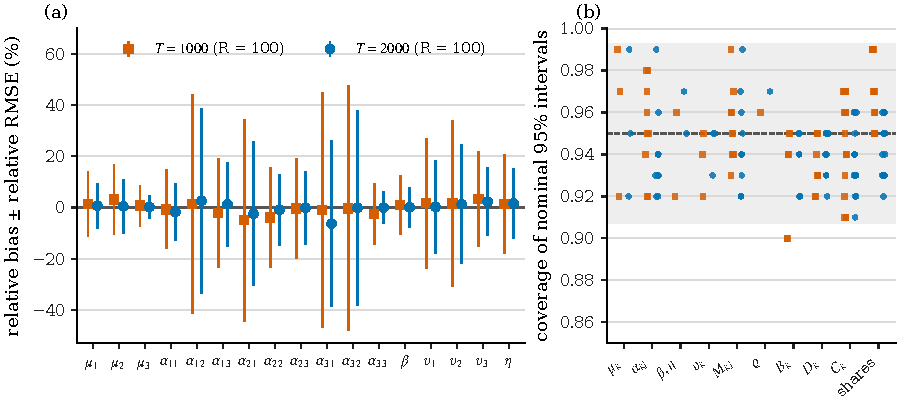
\includegraphics[width=6.0in]{figures/fig-sim-recovery.pdf}
\caption{E1, recovery by EM (synthetic data, $R=100$ per $T$). (a) Relative bias
(markers) $\pm$ relative RMSE (bars), in per cent, for the 17 parameters. (b) Coverage of
nominal $95\%$ intervals for the parameters and the derived quantities: multiplier entries
$M_{kj}$, spectral radius $\varrho$ and the surge components of E5. The grey band is the
$95\%$ Monte Carlo range around $0.95$ for $R=100$.}
\label{fig:sim-recovery}
\end{figure}

\begin{figure}[tbp]
\centering
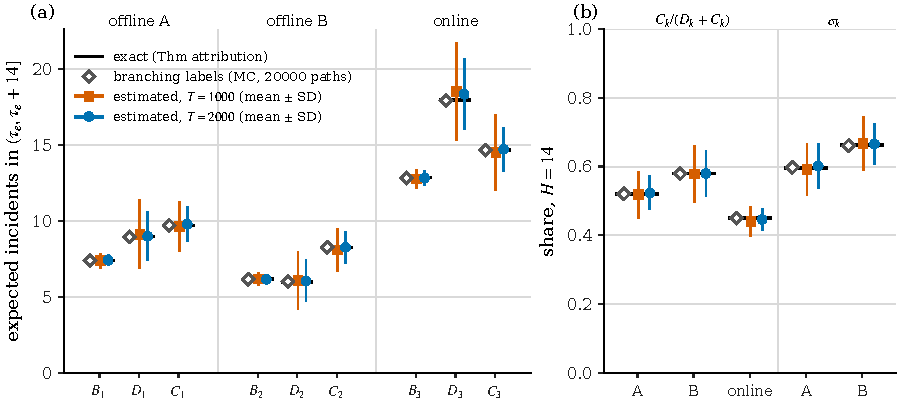
\includegraphics[width=6.0in]{figures/fig-sim-attribution.pdf}
\caption{E5, surge attribution after an event of size $S_e=3$ (synthetic data). (a) Expected
counts in $(\tau_e,\tau_e+14]$ by stream: exact values (\cref{thm:attribution}; lines),
branching-label Monte Carlo means (20{,}000 paths; diamonds), and estimates from the E1 fits
(mean $\pm$ SD over 100 replicates). (b) Contagion shares $C_k/(D_k+C_k)$ and online-channel
shares $\sigma_k$ at $H=14$, by stream.}
\label{fig:sim-attribution}
\end{figure}

\begin{figure}[tbp]
\centering
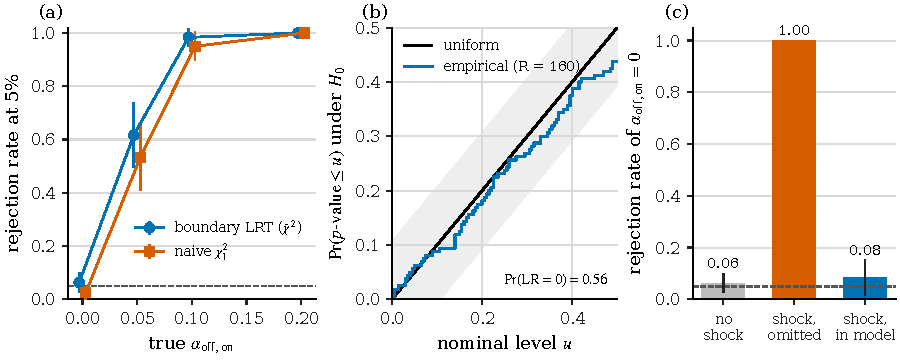
\includegraphics[width=6.0in]{figures/fig-sim-lrt.pdf}
\caption{E4, the test of $\alpha_{\mathrm{off},\mathrm{on}}=0$ (synthetic data; bars
$\pm1.96$ MC SE). (a) Rejection rate at the $5\%$ level against the true
$\alpha_{\mathrm{off},\mathrm{on}}$, for the chi-bar-square and the naive $\chi^2_1$
reference. (b) Empirical distribution function of the chi-bar-square $p$-values under
$H_0$ ($R=160$), with a $95\%$ Kolmogorov--Smirnov band; the $p$-value is $1$ whenever the
statistic is $0$. (c) Rejection rates without shocks, and with common shocks omitted from
or included in the model ($R=60$).}
\label{fig:sim-lrt}
\end{figure}

\FloatBarrier
\subsection{Monte Carlo standard errors}\label{app:sim-mcse}

Let $x_1,\dots,x_R$ be the estimates of a quantity with true value $x_0$ over $R$
replicates, with mean $\bar x$, standard deviation $s_x$ and errors $\varepsilon_r=x_r-x_0$.
\begin{itemize}
  \item \emph{Mean and bias.} The bias is $\bar x-x_0$. The MC SE of the mean and of the
  bias is $s_x/\sqrt R$. Medians are reported without MC SE.
  \item \emph{RMSE.} $\mathrm{RMSE}=(R^{-1}\sum_r\varepsilon_r^2)^{1/2}$, with MC SE
  $s_{\varepsilon^2}/(2\,\mathrm{RMSE}\sqrt R)$ by the delta method, where
  $s_{\varepsilon^2}$ is the standard deviation of the squared errors.
  \item \emph{Coverage and rejection rates.} For an estimated proportion $\hat\pi$, the
  MC SE is $\{\hat\pi(1-\hat\pi)/R\}^{1/2}$. The band of \cref{fig:sim-recovery}(b) is
  $0.95\pm1.96\,(0.95\times0.05/R)^{1/2}$.
  \item \emph{E5.} For each quantity, the mean over the $N=20{,}000$ paths has MC SE
  $(\hat\sigma^2/N)^{1/2}$, with $\hat\sigma^2$ the sample variance over paths, and
  $z=(\text{mean}-\text{exact})/\text{MC SE}$.
  \item \emph{E6.} Costs per window, Brier, CRPS and log scores and the mean forecast bias
  are averaged within each replicate; the MC SE is the standard deviation of the 12
  replicate averages divided by $\sqrt{12}$. Differences between two forecasters are
  paired: the MC SE is that of the 12 replicate differences. Alert rates, precision and
  recall are pooled over all 1800 windows and have no reported MC SE. The PIT statistic is
  $\chi^2=\sum_{b=1}^{10}(h_b-e)^2/e$, with $h_b$ the bin counts and $e$ the number of
  windows divided by 10, referred to $\chi^2_9$. The windows do not overlap and the outcomes
  are settled, so by \cref{lem:fc-pit}(b) the PIT values are independent under a correct
  forecast; the reference ignores the Monte Carlo error of the predictive distributions.
  The state ratios are ratios of means over all windows.
\end{itemize}
In the figures, error bars are $\pm1.96$ MC SE, except in \cref{fig:sim-recovery}(a)
($\pm$ relative RMSE), \cref{fig:sim-attribution} ($\pm1$ SD over replicates) and
\cref{fig:sim-thinning}(c) (no bars).

\subsection{Reproduction}\label{app:sim-repro}

From \texttt{papers/contagion/code/}, the commands
\begin{quote}\small
\texttt{OPENBLAS\_NUM\_THREADS=1 nice python run\_experiments.py -{}-workers 2}\\
\texttt{python make\_figures.py}
\end{quote}
run all six experiments, write \texttt{results/raw/E*.json} and
\texttt{results/sim\_results.json}, and then the figures and the tables
\texttt{tables/tab-sim-e1.tex}, \dots, \texttt{tab-sim-e6.tex}. With the current driver a
single run replaces the steps of \cref{app:sim-run}: E5 uses 20{,}000 paths, E2 includes
the long windows, E3 the three error levels and E6 the integrating forecasters, and the
seeds of every value stored earlier are unchanged. One experiment can be rerun with
\texttt{-{}-only E5} (E5 reads the stored E1 results when E1 is not run in the same
invocation); \texttt{-{}-augment-e2} repeats revision step (4); and
\texttt{-{}-merge-only} rebuilds the results file from the raw files. The option
\texttt{-{}-quick} runs tiny configurations in seconds; the tests in
\texttt{code/tests/test\_experiments.py} use it to check the output schema, the absence of
failed replicates, that two runs give identical results and that the integrating
forecasters leave the other E6 forecasters unchanged. With the recorded software versions,
the seeds determine every replicate. We have not checked whether other versions of NumPy or
SciPy reproduce the results to the last digit.
